\documentclass{report}
\usepackage[round]{natbib}
\usepackage{fullpage}
\usepackage{graphicx}
\usepackage[utf8]{inputenc}
\usepackage{listings}
\usepackage{mathtools, bm}
\usepackage{amssymb, bm}
\usepackage[hidelinks]{hyperref}

\renewcommand*\d{\mathop{}\!\mathrm{d}}
\renewcommand\phi{\varphi}
\renewcommand\O{\mathcal{O}}

\def\ssq{\subseteq}
\def\N{\mathbb{N}}
\def\R{\mathbb{R}}
\def\T{\mathcal{T}}
\def\iso{\text{iso}}
\def\ani{\text{ani}}

\begin{document}

\bibliographystyle{plainnat}
\lstset{language=Matlab}

\title{Heat and Color Flow with Finite Elements}
\author{Obed Afram, Anissa El Keurti, Robert Seidel}
\date{November 2016}
\maketitle

\chapter{The Poisson Equation with Finite Elements}

\chapter{Anisotropic Diffusion using Finite Element Method}

After applying the Finite Element Method to common and abstract cases, we chose to work on a diffusion equation which is applied in image processing. A typical problem in image processing is \emph{denoising}. One way to remove noise in a picture is to blur noisy areas while leaving edges unchanged. The linear heat equation can be used to blur an image, as the flow of heat can be interpreted as a flow of color on a plate. However, the linear heat equation does not preserve edges. In this project, we study the effects of a nonlinear PDE in image processing: the Perona-Malik anisotropic diffusion equation, that slows down the diffusion on domains where an edge has been detected. We explain our Finite Element solver for that problem and display various numerical experiments.

\section{What is a picture?}

L infty
derivative
grad u as edge indicator

\section{The Perona-Malik Equation and Finite Elements}

\subsection{Diffusion Equation}

The Perona-Malik equation \citep{perona1990} is a nonlinear diffusion equation that uses an inhomogeneous diffusivity coefficient,
\begin{equation} \label{pm}
	u_t = \nabla \cdot \left( g(\|\nabla u\|) \nabla u \right),
\end{equation}
where typical choices for $g$ are
\begin{equation}
	g(\|\nabla u\|) = e^{-(\|\nabla u\|/K)^2}
\end{equation}
or
\begin{equation}
	g(\|\nabla u\|) = \frac{1}{1 + \left( \frac{\|\nabla u\|}{K}\right)^2}.
\end{equation}
Apparently, image areas with a small gradient experience strong blurring while edge areas remain unchanged. The original formulation (\ref{pm}) can lead to local backwards diffusion and become an ill-posed problem. Thus, we employ the so called \emph{regularized} Perona-Malik equation as proposed by \cite{catte1992}, where the edge indicator $\|\nabla u\|$ is replaced by $\|\nabla (G_\sigma \ast u)\|$, $G_\sigma \in C^\infty(\R^2)$ a smoothing kernel. The rest of this section relies on the definitions as given in \cite{handlovicova2002}. We begin with the regularized Perona-Malik equation
\begin{equation} \label{pmreg}
    u_t = \nabla \cdot \left( g\left(\left\|\nabla (G_{\sigma} \ast u)\right\|\right) \nabla u \right).
\end{equation}

The function $u = u(t,x)$ is defined in $I \times \Omega$. We assume $I = [0, T]$ and $\Omega \ssq \R^2$ to a bounded rectangular domain. The parameter $t$ can be seen as abstract scaling parameter \citep[p. 219]{handlovicova2002}. We equip (\ref{pmreg}) with Neumann boundary conditions
\begin{align}
	\frac{\partial u}{\partial \nu} &= 0 & \text{on } I \times \partial \Omega, \\
	u(0,x) &= {u^0}(x) & \text{in } \Omega.
\end{align}

Further, we assume $g: \R^+ \rightarrow \R^+$ to be a smooth, nonincreasing function, $g(0)=1$ and $\lim_{s \rightarrow \infty} g(s) = 0$. For the smoothing kernel, we assume $G_\sigma \in C^\infty(\R^2)$, $\int_\R G_\sigma \d x = 1$, $\int_\R |G_\sigma| \d x < \infty$ and that $G_\sigma$ converges to the Dirac measure if $\sigma \to 0$. Finally, let $u^0 \in L^\infty(\Omega)$. As described in \cite{handlovicova2002}, we do not compute the convolution $G_{\sigma} \ast u$, but use isotropic diffusion, i.e. $g \equiv 1$, in order to obtain a blurred version $u_iso$ of the image. The PDE simplifies in this case to
\begin{equation} \label{pmiso}
	\frac{\partial u_\iso}{\partial t} = \Delta u_\iso.
\end{equation}

\subsection{Finite Element Method} 

We do not present the full derivation of the Finite Element procedure in this report, but refer to the lecture and the paper from \cite{handlovicova2002}. The linear isotropic solution $u_\iso$ is used to compute the diffusion coefficients $g\left(\left\|\nabla (G_{\sigma} \ast u)\right\|\right)$. We assume these coefficients as fixed in scale, i.e. we numerically compute
\begin{equation}
	\frac{\partial u_\ani}{\partial t} = \nabla \cdot (\underbrace{g(\|\nabla \underbrace{(G_{\sigma} \ast u^0)}_{=u_\iso}\|)}_\text{const.} \nabla u_\ani).
\end{equation}

We use implicit Euler in scale and obtain the weak formulations
\begin{align}
	\int_\Omega u_\iso v \d x + \sigma \int_\Omega \nabla u_\iso \nabla v \d x &= \int_\Omega u^0 v \d x, \\
	\int_\Omega u_\ani v \d x + \tau \int_\Omega g(\|\nabla u_\iso\|) \nabla u_\ani \nabla v \d x &= \int_\Omega u^0 v \d x.
\end{align}

We consider a triangulation $\T_h$ of $\Omega$ and a nodal basis of continuous, piecewise linear functions $\phi_j$, satisfying $\phi_j(x_i) = \delta_{ji}$ for all nodes $x_i$ of $\T_h$, $i,j=1,...,M$. The initial value $u^0$ and the unknown functions $u_\iso$ and $u_\ani$ are represented by
\begin{align}
	u^0_h & = \sum_{i=1}^{M} u^0_i \phi_i, \\
	u_{\iso, h} &= \sum_{i=1}^{M} u_{\iso, i} \phi_i, \\
	u_{\ani, h} &= \sum_{i=1}^{M} u_{\ani, i} \phi_i,
\end{align}
with the unknown scalar coefficients $u^0_i, u_{\iso, i}, u_{\ani, i} \in \R$, $i=1,...,M$. With the Ritz-Galerkin method, we obtain
\begin{align}
	\sum_{i=1}^{M} \left( \int_\Omega \phi_i \phi_j \d x + \sigma \int_\Omega \nabla \phi_i \nabla \phi_j \d x \right) u_{\iso, i} &= \sum_{i=1}^{M} \left( \int_\Omega \phi_i \phi_j \d x \right) u^0_i, \\
	\sum_{i=1}^{M} \left( \int_\Omega \phi_i \phi_j \d x + \tau \int_\Omega g(\|\nabla u_{\iso,h}\|) \nabla \phi_i \nabla \phi_j \d x \right) u_{\ani, i} &= \sum_{i=1}^{M} \left( \int_\Omega \phi_i \phi_j \d x \right) u^0_i.
\end{align}

This can also be written as two linear systems
\begin{align}
	M + \sigma A(1) &= M u^0_h, \\
	M + \tau A(g(\|\nabla u_{\iso,h}\|)) &= M u^0_h,
\end{align}
where $M_{j,i} = \int_\Omega \phi_i \phi_j \d x$ is the so-called \emph{mass matrix} and $A(w)_{j,i} = \int_\Omega w \nabla \phi_i \nabla \phi_j \d x$ is the \emph{stiffness matrix}. The parameters $\sigma$ and $\tau$ denote the scale parameter for the two diffusion processes.

\section{Numerical experiments}

\subsection{First steps} 

We performed several numerical simulations of the Perona-Malik diffusion using the Finite Element Method on 2D images. Our first sample is the \texttt{cameraman} picture, see Figure \ref{cameraman}. We just write $u^0 \in \R^{n_1 \times n_2}$ from now on, to denote the initial data, where $n_1, n_2 \in \N$ denote the image dimensions.

NOISE GENERATION

We use a noisy image (by adding a random noise of parameter ${\sigma}_{noise}$) and we choose the scale of the initial image. In the figure \ref{g1-1}, the first image in the left represents the initial image that has been rescaled and added noise. The second image shows the mesh grid. Finally the two last images use two different interpolation methods on the grid, that will be developed later. \\

\subsubsection{Triangular Mesh}

A naive approach for the grid generation is to identify each pixel in the image with a node on the grid. The obtained squares are crossed diagonally to obtain triangles. This procedure yields a grid with $\O(n_1 n_2)$ nodes and $\O(2 n_1 n_2)$ elements. It turns out handy to use the matrix indices as spatial coordinates, i.e. we set $\Omega = [1,n_1] \times [1,n_2]$ and in the triangulation $x_{i,j} = (i,j)$ for $i=1,...,n_1$, $j=1,...,n_2$.
 
The function, that we called "getSquareTri" takes the dimensions of the picture as a variable and returns: 
\begin{itemize}
    \item
    p: the set of all the nodes's $(i,j)$ coordinates 
    \item
    tri: the set of all the triangles in the grid
    \item
    edge: the set of all the edges in the grid 
\end{itemize}
 

 
 
 %% the mask apply function
 
 

\begin{figure}[h!]
\centering
\begin{tabular}{|p{1cm}|p{1cm}|p{1cm}|}
  \hline

  $(1,1)$ &    & $(n_1,1)$  \\
 \hline
  $(1,n_2)$ &  & $(n_1,n_2)$\\
  \hline
\end{tabular}
\end{figure}


 
 \begin{figure}[h!]
\label{g1}
 \centering
 \includegraphics[scale=0.7]{g1.jpg}
 \end{figure}
 
 
 

 
 
 
 
 
 \begin{figure}[h!]
 \label{g1-1}
 \caption{Visualization of the grid with ${\sigma}_{noise}=0.05$ and $scale=0.1$}
 \centering
 \includegraphics[scale=0.7]{g1-1.jpg}
 \end{figure}








\subsubsection{Algorithm}

The first program we performed uses the same method that was used in the part 1 of the project. First, compute the meshgrid and 

It takes the following arguments: 
\begin{itemize}
    \item
    u: the initial noisy and rescaled image 
    \item 
    tri, p, edge (output of the getSquareTri function)
    \item
    the parameters $\sigma$ and $\tau $
    \item
    The diffusion coefficient (that we call transfer function) g
\end{itemize}


And it returns the followings elements: % à compléter 
\begin{itemize}
    
    \item 
    $u_{ani}$: the anisotropic solution
    \item
    The matrix $A_{iso}$
    \item
    The matrix M
    \item
   $ u_{iso}$: the isotropic solution (solution of the first system)
    \item
    $g_{ani}$
    \item
    The matrix $A_{ani}$
\end{itemize}



The algorithm works in the following way: \\

\underline{Isotropic diffusion}
\begin{enumerate}
    
    \item 
    Initialization of M, $A_{iso}$, $A_{ani}$
     \item 
     For each triangle (visited once):
     \begin{itemize}
          \item
          Get the node ID to identify points and basis function
          \item 
          Get the coordinates of the points (p1,p2,p3) 
          \item 
          Compute the function $\phi_i$ that land in the triangle
          \item 
          For i from 1 to 3: 
          For j from 1 to 3: 
          \begin{itemize}
          \item
              We compute $f_{iso} = \sum {\phi_i \phi_j}$ to calculate then the integral of $f_{iso}$ thanks to the quadrature2D (programmed in the first part) 
          \item
              $A_{iso}(nodeID(i),nodeID(j)) =  A_{iso}(nodeID(i),nodeID(j)) + quadrature2D (p1,p2,p3,Nq,f_{iso})$
          \item
              We compute $f_{mass} = \sum {\phi_i(x,y) \phi_j(x,y)}$
          \item
              $M(nodeID(i),nodeID(j)) =  M(nodeID(i),nodeID(j)) + quadrature2D(p1,p2,p3,Nq,f_{mass})$
          \end{itemize}
     \end{itemize}
     \item 
     Resolve: $(M + \sigma A_{iso}) u_{iso} = M u$
\end{enumerate}




\underline{Anisotropic diffusion}
\begin{enumerate}

    
    \item 
    Initialization of the diffusion coefficient d
     \item 
     For each triangle (visited once):
     \begin{itemize}
          \item
          Get the node ID to identify points and basis function
          \item 
          Get the coordinates of the points (p1,p2,p3) 
          \item 
          Compute the function $\phi_i$ that land in the triangle
          \item 
          Compute $d(k) = d(k) + u_{iso}(nodeID(i)) \phi_i$
          \item 
          Compute the transfer function: $g=(|d|)$
          \item 
          For i from 1 to 3: 
          For j from 1 to 3: 
          \begin{itemize}
          \item
              We compute $f_{ani} = g(k) \sum {\phi_i \phi_j}$ to calculate then the integral of $f_{ani}$ thanks to the quadrature2D (programmed in the first part) 
          \item
              $A_{ani}(nodeID(i),nodeID(j)) =  A_{ani}(nodeID(i),nodeID(j)) + quadrature2D (p1,p2,p3,Nq,f_{ani})$
         
          \end{itemize}
          
     \end{itemize}
     \item 
     Resolve: $(M + \tau A_{ani}) u_{ani} = M u$
\end{enumerate}



\subsubsection{Results}


\underline{Parameters}

We chose the following parameters for the first simulations: 
\begin{itemize}
\item
$\sigma=0.5$
\item
$\tau=1.5$
\item
The tranfer function: $g= exp(-(10*x)^2)$ \\
\end{itemize}


\underline{Visualization} 


In order to have a complete visualization of the results, we chose to output four pictures: 
\begin{enumerate}
\item 
The first picture is the initial picture (noisy and rescaled)
\item
The second picture shows the grid (nodes, elements and positions)
\item
The third picture is a visualization of the isotropic solution $u_iso$ (only on the grid points). We used the "Interpolated Shading" from Matlab to give a smooth result. 
\item
The fourth picture represents the anisotropic solution $u_ani$ interpolated on all the pixels. We used the function "griddata" and the method "natural". 
\end{enumerate}




Our program is very slow (see the table \ref{T1} for more precisions) and uses many nodes even if the result is satisfying:less noise and edges preserved (see the figure \ref{t1}). We also calculate also the PSNR by taking the initial rescaled image without noise as a reference. The PSNR (peak signal to noise ratio) is a tool that allows us to measure the quality of our reconstruction. 





\subsection{Efficient implementation}

\subsubsection{Method}

In order to make a more efficient implementation, we took the following measures:

\begin{itemize}
    \item
    Precomputation and storage of triangle areas, basis function coefficients and triangle midpoints.
    The triangles areas: for each triangle, each area is computed beforehand. 
    \item 
    Enforce more use of vector notation.
    \item 
    Removal of the function call of \texttt{quadrature2D} and an anonymous function call. Instead, we used the precomputed values to get the triangular integral.
\end{itemize}


\subsubsection{Results}

The program obtained is faster than the previous one (see details in figures \ref{T2} ). 

         \begin{figure}[h!]
         	\centering
         	\label{T2}
         	\begin{tabular}{|c|c|}
         		\hline
         		Duration &  Precomputation: 0.85s,
         		Isotropic diffusion: 5.97s,
         		Anistropic diffusion:2.7 s   \\
         		\hline
         		Number of nodes & 16384 \\
         		\hline
         		Number of elements & 32258\\
         		
         		\hline
         		PSNR & 27.36 \\
         		\hline
         	\end{tabular}
         	\caption{Table of results with the pre-computed program : scale=0.5, $\sigma_{noise}=0.05$, $\sigma=0.5$, $\tau=1.5$ }
         \end{figure}

%%% t1: test with test_pm_tri (and getSquareTri) + scale 0.5

\begin{figure}[h!]
	\centering
	\label{t1}
	\caption{Visualization with: scale=0.5, $\sigma_{noise}=0.05$  $\sigma=0.5$, $\tau=1.5$ }
	\includegraphics[scale=0.8]{t1.jpg}
\end{figure}

%table of results 
\begin{figure}[h!]
	\caption{Table of results with: scale=0.5, $\sigma_{noise}=0.05$  $\sigma=0.5$, $\tau=1.5$ }
	\centering
	\label{T1}
	\begin{tabular}{|c|c|}
		\hline
		Duration &  Isotropic diffusion: 49.6 s
		and Anistropic diffusion:27 s   \\
		\hline
		Number of nodes & 16384 \\
		\hline
		Number of elements & 32258\\
		\hline
		PSNR & 27.64\\
		\hline
	\end{tabular}
\end{figure}

        % t2.jpg test_pm_tri_pre and getSquareTri, scale=0.5, sigma=0.05
        \begin{figure}
        \label{t2}
        \caption{Visualization of $u_{ani}$ with the pre-computed program : scale=0.5, $\sigma_{noise}=0.05$  $\sigma=0.5$, $\tau=1.5$ }
        \centering
        \includegraphics[scale=0.8]{t2.jpg}
        \end{figure}








\subsection{Grid generation strategies}


\subsubsection{Swap the triangles}
\underline{Method}

In order to fit better the edges of the image, we decided to proceed to a regularization technique by swapping the diagonals of some triangles. 
For each square, we compare these two terms:
$|value_{Top Left} - value_{Bottom Right}|$ and $|value_{Top Right}- value_{Bottom Left}|$. If the first term is higher than the second term, we swap the triangles. For the "Cameraman" picture, with $scale=0.1$ we obtain the grid on the figure \ref{g2}. \\

Then, we applied the grid for the Perona-Malik diffusion using the pre-computed version of the code. 






\underline{Results}

When we compare the results with the first grid, we notice that the new grid seems to be more adapted to the image (in the figure \ref{g1}, we can see "diagonal lines" that marks the triangles diagonals). \\

        % g2.jpg test_getSquareTri_swp for scale=0.1
        \begin{figure}
        	\label{g2}
        	\centering
        	\caption{Visualization of the "Swap Diagonal" grid for $scale=0.1$, and $\sigma_{noise}=0.05$}
        	\includegraphics[scale=0.8]{g2.jpg}
        \end{figure}


        %t3 test_pm_tri_pre with getSquareTri_swp scale=0.5
        \begin{figure}
        \label{t3}
        \centering
        \caption{Visualization of $u_{ani}$ with: the "Swap Diagonal" grid, $scale=0.5$, $\sigma_{noise}=0.05$,$\sigma=0.5$, $\tau=1.5$}
        \includegraphics[scale=0.8]{t3.jpg}
        \end{figure}





        \begin{figure}[h!]
        \centering
         \caption{Table of results with: the "Swap Diagonal" grid, $scale=0.5$, $\sigma_{noise}=0.05$,$\sigma=0.5$, $\tau=1.5$}
        \label{T3}
        \begin{tabular}{|c|c|}
          \hline
         Duration &  Precomputation: 0.78s,
         Isotropic diffusion: 5.46s,
         Anistropic diffusion:2.45 s   \\
        \hline
         Number of nodes & 16384 \\
         \hline
         Number of elements & 32258\\
 
         \hline
         PSNR & 27.19 \\
         \hline
        \end{tabular}
        \end{figure}







\subsubsection{Using the variance}
\underline{Method}

% on utilise aussi gaussian filter ici 

In order to use less elements in the smooth areas, and more elements in the edge areas we decided to perform a new grid by using a variance criterion. We implemented a recursive function: the square is splitted in four other squares when the variance of the portion is higher than a certain value and then we apply a Delaunay triangulation to the points obtained by using the function "delaunayTriangulation". We also use a corner value criterion: if any of the square's edges or the two diagonals is higher than a certain value, we split. We use the both criteria to decide if we split or not the square.  But to use this method properly, we apply first to the image a Gaussian filter (function "imgaussfilt" in Matlab with parameter $\sigma_{GaussFilt}$) to blur the initial image (and the degree of blur depends on $\sigma_{GaussFilt}$) before applying the criteria.  \\







        % g3.jpg test_getVariGrid(U,sigma=1,minvar=0.003,cvc=0.05,alldepth=3,maxdepth=50) for scale=0.1 
        \begin{figure}
        \label{g3}
        \centering
        \caption{Visualization of the "Variance" grid, $scale=0.1$, $\sigma_{noise}=0.05$}
        \includegraphics[scale=0.8]{g3.jpg}
        \end{figure}
        
        
        
        
\underline{Results}

The result given seems satisfying regarding the few numbers of nodes and elements (see figures \ref{t4} and  \ref{T4}) that are used for the reconstruction. The picture is smooth but it is difficult to distinguish the edges. 

% Show four pictures 

        %t4 test_pm_tri_pre with getVariGrid(U,sigma=2,minvar=,cvc=,alldepth=,maxdepth=) scale=0.5 
        \begin{figure}[h!]
        \label{t4}
        \centering
        \caption{Visualization of $u_{ani}$ with: the "Variance" grid, $scale=0.5$, $\sigma_{noise}=0.05$,$\sigma=0.5$, $\tau=1.5$}
        \includegraphics[scale=0.8]{t4.jpg}
        \end{figure}
        

% Table of results 

        \begin{figure}[h!]
        \centering
        \label{T4}
        \caption{Table of results with: the "Variance" grid, $scale=0.5$, $\sigma_{noise}=0.05$,$\sigma=0.5$, $\tau=1.5$}
        \begin{tabular}{|c|c|}
          \hline
         Duration &  Precomputation: 0.13s,
         Isotropic diffusion: 0.75,
         Anistropic diffusion:0.33 s   \\
        \hline
         Number of nodes & 135 \\
         \hline
         Number of elements & 259\\
 
         \hline
         PSNR & 23.88 \\
         \hline
        \end{tabular}
        \end{figure}






\subsubsection{Using the gradient}
\underline{Method}


We decided to also try a gradient criterion to create the grid. 
We use matrix convolutions (function "conv2" in Matlab) to compute the vertical and horizontal derivatives. Then we normalize the gradient obtained in order to have a number between 0 and 1, and to use it as a probability to be a node. We create a gradient mask with the nodes selected and we apply a Delaunay triangulation (delaunayTriangulation). But to use this method properly, we apply first to the image a Gaussian filter (function "imgaussfilt" in Matlab with parameter $\sigma_{GaussFilt}$) to blur the initial image (and the degree of blur depends on $\sigma_{GaussFilt}$) before applying the gradient mask. We also apply a "transfer function" $g_{grad}$ to the norm of the gradient before selecting the nodes. 




        % g4.jpg test_getGradGrid(U,sigma=2, g=power(x,1)) for scale=0.1 
       \begin{figure}[h!]
       
        \centering
        \caption{Visualization of the "Gradient" grid, $scale=0.1$, $\sigma_{noise}=0.05$, $\sigma_{GaussFilt}=2$,  $g_{grad}=x$}
        \includegraphics[scale=0.8]{g4.jpg}
        \end{figure}
        


\underline{Results}

Using the "Gradient" grid gives a deeply smooth image. It results from the fact that we use the gradient twice in our analysis (once in the Perona-Malik diffusion equation, and once for the "Gradient" grid). Again, few nodes are used (see figure \ref{T5} for details). 



% Figure showing the final image 

        %t5 test_pm_tri_pre with test_getGradGrid(U,sigma=2, g=power(x,1)) for scale=0.5 
        \begin{figure}[h!]
        
        \centering
        \caption{Visualization of $u_{ani}$ with: the "Gradient" grid, $scale=0.5$, $\sigma_{noise}=0.05$,$\sigma=0.5$, $\tau=1.5$}
        \includegraphics[scale=0.8]{t5.jpg}
        \end{figure}





% Table of results 

        \begin{figure}[h!]
        \centering
        \caption{Table of results with: the "Gradient" grid, $scale=0.5$, $\sigma_{noise}=0.05$,$\sigma=0.5$, $\tau=1.5$}
        \label{T5}
        \begin{tabular}{|c|c|}
          \hline
         Duration &  Precomputation: 0.11s,
         Isotropic diffusion: 0.63,
         Anistropic diffusion:0.28 s   \\
        \hline
         Number of nodes & 197 \\
         \hline
         Number of elements & 374\\
 
         \hline
         PSNR & 22.1 \\
         \hline
        \end{tabular}
        \end{figure}






\subsection{Parameter modification}
\subsubsection{The time $\tau$}


We wanted to see the diffusion on the picture for different values of $\tau$ (figure \ref{t6}). We compare the PNSR (figure \ref{T6}) between the different values and $\tau=1.5$ seems to be the best choice, even when we compare it with other close values ($\tau=2$,$\tau=2.5$,$\tau=3$ ...). \\ 


        %t6 test_pm_tri_preTau with sigma=0.5 and g idem
        \begin{figure}
        \label{t6}
        \centering
        \caption{Visualization of the diffusion for different $\tau$ with $scale=0.5$, $\sigma_{noise}=0.05$,$\sigma=0.5$ }
        \includegraphics[scale=0.2]{t6.jpg}
        \end{figure}
        




% Table of results 

        \begin{figure}[h!]
        \label{T6}
        \centering
         \caption{Table of results for different $\tau$ with $scale=0.5$, $\sigma_{noise}=0.05$,$\sigma=0.5$ }
        \begin{tabular}{|c|c|c|c|c|c|c|c|}
        \hline
        Method & $\tau=0$ & $\tau=1.5$ & $\tau=5$ & $\tau=5$ & $\tau=10$ & $\tau=50$ & $\tau=100$
        \\ \hline
         PSNR  & 26.4 & 27.22 & 25.39 & 24.23 & 21.43 & 20.27 \\
         \hline
        \end{tabular}
        \end{figure}






\subsubsection{The coefficient $\sigma$}

Then, we wanted to study the effects of the parameter $\sigma$ from the diffusion equation on the picture. We compare the PSNR for the different values of $\sigma$ and the best choice seems to be $\sigma=0$ (see figures \ref{t7} and \ref{T7}). When we compare this choice with other close values ($\sigma=0.1$,$\sigma=0.2$...) we obtain the same result. 

        %t7 test_pm_tri_preSigma with tau=1.5
         \begin{figure}
         \label{t7}
        \centering
        \caption{Visualization of the diffusion for different $\sigma$ with $scale=0.5$, $\sigma_{noise}=0.05$,$\tau=1.5$ }
        \includegraphics[scale=0.2]{t7.jpg}
        \end{figure}
        
       



 \begin{figure}[h!]
        \centering
        \label{T7}
         \caption{Table of results for different $\sigma$ with $scale=0.5$, $\sigma_{noise}=0.05$,$\tau=1.5$}
        \begin{tabular}{|c|c|c|c|c|c|c|}
        \hline
        Method & $\sigma=0$ & $\sigma=1.5$ & $\sigma=5$ & $\sigma=10$ & $\sigma=50$ & $\sigma=100$ \\
        \hline
        PSNR  & 30.2 & 27.3 & 24.42 & 23.8 & 23.26 & 22.8 \\
        \hline
        \end{tabular}
        \end{figure}







\subsubsection{Transfer function}


The modification of the diffusion coefficient, or more precisely the transfer function $g$ can change the way the diffusion processes on the image. We tested several transfer functions that are non-increasing and whose the limit tends toward 0. The choice of the transfer function depends on the application (deleting the noise or keeping the details for example). According to the comparison between the PSNR, the function $g= e^{-{100 x}^2}$ seems to be the best choice (see figure \ref{t8}), the picture keeps many details but is still noisy. The function $g= e^{-{10 x}^2}$ seems to give a good result with a smooth image.  \\


%https://books.google.no/books?id=JykChzLVlogC&pg=PA4&lpg=PA4&dq=anisotropic+diffusion+%22transfer+function%22&source=bl&ots=Z3VKxCW-hy&sig=NcAAOPtQ6p_ngSGSEs5GYRoLgdA&hl=fr&sa=X&ved=0ahUKEwjQ5aj0rI_QAhWE3SwKHWGnCp8Q6AEIYTAJ#v=onepage&q=anisotropic%20diffusion%20%22transfer%20function%22&f=false
%We can also use, fonction continue par morceaux -> for medical data. Depends on what we want regarding the edges etc 







% function imDifffCoeff -> plots g coeff but only on structured grids



\subsubsection{Interpolation}

We tried to modify the visualization of our results by changing the interpolation method for the anisotropic solution ("natural","nearest","linear","cubic","v4"). However we don't see any particular differences between the different interpolation methods with the "cameraman" picture. 




\subsubsection{The parameters of the grids}

For the "Variance" and "Gradient" grid, the numbers of nodes and elements are very low regarding the quality of the image. We can modify the parameters in order to increase the numbers of nodes and elements. 
For the "Variance" grid (see figure \ref{t11}), we decrease the "minimum variance" value, so more nodes can be selected. For the "Gradient grid" (see figure \ref{t12}) we can only modify the function $g_{grad}$ that we defined earlier. 






\subsubsection{The noise}


We wanted to study the different effects of our grids when we increase the noise in the initial picture. So far, if we compare the "ratio" $\frac{PSNR}{NumberOFElement}$ (important for the algorithm's speed), the grids "Variance" and "Gradient" have the best ratio.For a very noisy picture ($\sigma_{noise}=0.2$) we compare the visualizations obtained (figure \ref{t13}). We notice that the "gradient" grid has a less good quality than the other grids, the final picture seems to be even more noisy than the initial one.  







\subsection{Quadrilateral elements}

\underline{Method}

Instead of using triangles, we thought we could use squares. We performed a Finite element algorithm using squares instead of the triangles. We used analytical computations to make the code faster by computing: 

\begin{itemize}
    \item 
    The $\phi_i$ functions and their value on the integration point 
    \item 
    The integration of the $\phi_i$ functions 
    
\end{itemize}

The visualization shows: 
\begin{enumerate}
\item 
The initial noisy image ($scale=0.5$)
\item 
The isotropic solution 
\item 
The anisotropic solution
\end{enumerate}



\underline{Results}

We notice a "checkerboard" effect (figure \ref{t14} and \ref{T14}) on the visualization of the anisotropic solution. The article \cite{Shukla13} explains that the "checkerboard" effect is a common problem of the finite element method. One way to resolve it is to use a higher order finite element but that leads to more expensive program. Other methods are proposed like "the perimeter control technique", or "the patch technique" etc. 



\section{Outlook}

Our work can be applied in several fields that involve image processing. In the medical field, image processing is often used to read information from ultrasound images for example. The goal is to distinguish the layers of different tissues (in order to find a tumor for example), this can be relatively difficult when the image is very noisy. \\

We can, in a future work, apply our algorithm on 3D images or use a higher order finite element method. \\



\chapter*{Conclusion}

In this work, we showed how to implement the Perona-Malik diffusion equation using Finite element methods with a relatively fast algorithm. We also showed how to reduce the numbers of elements and nodes (so the algorithm's speed) by focusing on the important zones (edges for example) by using different methods (variance and gradient). The comparison between the different methods leads to choices depending on the application chosen (medical data, picture restoration etc) since different factors have to be taken into account (quality, speed, smoothness). 

\chapter*{Appendix: Figures}

        %t8 test_pm_tri_preG with tau=1.5, s=0.5
        \begin{figure}
        	\label{t8}
        	\centering
        	\caption{Visualization of the diffusion for different $g$ with $scale=0.5$, $\sigma_{noise}=0.05$,$\tau=1.5$, $\sigma=0.5$ }
        	\includegraphics[scale=0.2]{t8.jpg}
        \end{figure}
        
        
        
        
        
        \begin{figure}[h!]
        	\centering
        	\label{T8}
        	\caption{Table of results for different $g$ with $scale=0.5$, $\sigma_{noise}=0.05$,$\tau=1.5$, $\sigma=0.5$ }
        	\begin{tabular}{|c|c|c|c|c|c|c|}
        		\hline
        		Method & $g= e^{-10 x}$ & $g= e^{-{0.5 x}^2}$ & $g= e^{-{10 x}^2}$ & $g= e^{-{100 x}^2}$ & $g= tanh(5 x)+1$ & $g= 1-x$  \\
        		\hline
        		PSNR  & 26.32 & 22.73 & 27.22 & 28.82 & 25.37 & 23.13 \\
        		\hline
        	\end{tabular}
        \end{figure}
        
        
        
        \begin{figure}
        	\centering
        	\label{t9}
        	\caption{Visualization of the diffusion for different interpolation methods with the "Swap triangles" grid and $scale=0.5$, $\sigma_{noise}=0.05$,$\tau=1.5$, $\sigma=0.5$ }
        	\includegraphics[scale=0.2]{t9.jpg}
        \end{figure}

\begin{figure}
	\centering
	\label{t11}
	\caption{Visualization of the diffusion for different "Variance grid" parameters with $scale=0.5$, $\sigma_{noise}=0.05$,$\tau=1.5$, $\sigma=0.5$ }
	\includegraphics[scale=0.2]{t11.jpg}
\end{figure}

\begin{figure}
	\centering
	\label{t12}
	\caption{Visualization of the diffusion for different "Gradient grid" parameters with $scale=0.5$, $\sigma_{noise}=0.05$,$\tau=1.5$, $\sigma=0.5$ }
	\includegraphics[scale=0.2]{t12.jpg}
\end{figure}



\begin{figure}[h!]
	\label{t13}
	\centering
	\caption{Visualization of the diffusion for different grids and $scale=1$, $\sigma_{noise}=0.2$,$\tau=1.5$, $\sigma=0.5$ }
	\includegraphics[scale=0.2]{t13.jpg}
\end{figure}

        %t9 test_pm_tri_tet_pre with tau=1.5, s=0.5
        \begin{figure}
        	\label{t14}
        	\centering
        	\caption{Visualization of the diffusion for a "squares" grids and $scale=0.5$, $\sigma_{noise}=0.05$,$\tau=1.5$, $\sigma=0.5$ }
        	\includegraphics[scale=0.2]{t14.jpg}
        \end{figure}
        
        
        
        \begin{figure}
        	\centering
        	\caption{Table of results for a "squares" grids and $scale=0.5$, $\sigma_{noise}=0.05$,$\tau=1.5$, $\sigma=0.5$ }
        	\label{T14}
        	\begin{tabular}{|c|c|}
        		\hline
        		Duration &  
        		Isotropic diffusion: 6.69s,
        		Anistropic diffusion:1.95 s   \\
        		\hline
        		Number of nodes & Number of pixels nx1*nx2 \\
        		\hline
        		Number of elements & (nx1-1)*(nx2-1)\\
        		\hline
        		PSNR & 16.12 \\
        		\hline
        	\end{tabular}
        \end{figure}

\begin{figure} \label{cameraman}
	\centering
	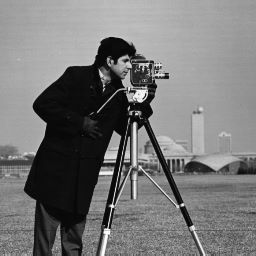
\includegraphics{cameraman.jpg}
	\caption{The \texttt{cameraman} picture}
\end{figure}

\bibliography{literature}


\end{document}
